
% MISSING PER THE GUIDE (needs new writing by you, not copy-paste):
%   - §3.6: a 3-5 line chapter-opening paragraph for this new Chapter 2
%     (guide says Ch.1 already has a usable opener; this one does not, since
%     the old Ch_3_pca.tex opener was written to introduce PCA specifically,
%     not the whole theory chapter — I left the old PCA-specific opening
%     text in place under §2.1 below rather than inventing a new one).
%============================================================================

\chapter{Machine learning theory}
\label{ch:ml_theory}

\section{Machine learning framework and problem setting}
\label{sec:ml_framework}

Machine learning is the field of study that gives computers the ability to learn from data without being explicitly programmed. In this context, a model is a mathematical function or computational structure that transforms input data into an output, following rules that are not explicitly defined but inferred from examples. The data are represented through numerical features, and the model uses them to learn relationships, trends or structures that are relevant for a given task, such as classification or dimensionality reduction. During training, the model adjusts its internal parameters according to the examples it receives, in order to capture patterns that remain informative when new observations are presented.

This approach is well suited to Raman spectroscopy of biological tissues. As discussed in \Cref{ch:introduction}, the complexity of biological Raman spectra makes it difficult to reduce the classification problem to a few manually selected bands. For this reason, the entire spectrum is treated as a numerical object whose overall profile may contain information relevant to the classification task. In the dataset used in this work, the Raman measurements are already organized in a computationally suitable tabular form. Starting from the structure described in \Cref{ch:Dataset}, the input data for the machine learning analysis are obtained from the spectral columns \texttt{band\_}n. These columns contain the Raman intensity values at the 483 selected shifts; from a machine learning perspective, they form the feature vector associated with each pixel-level spectrum acquired from a Raman map. When all spectra are considered together, the corresponding feature vectors are arranged into a data matrix, whose rows represent spectra and whose columns represent Raman-shift variables.

Machine learning methods are commonly distinguished according to the information available during training. When the aim is to train a classifier, the learning process is supervised: the model is shown both the input data and the correct output associated with each example. In this way, it can learn how spectral information is related to tissue classes and use this relation to assign a class to new spectra. In the present work, this corresponds to using each Raman spectrum as input and its associated tissue label as the target output for binary classification.

When labels are not part of the learning process, the analysis becomes unsupervised: the algorithm only receives the input data and searches for structure within them. This approach is useful when the goal is not to assign a class directly, but to explore the organization of the data, visualize similarities between spectra or reduce the number of variables.

This chapter focuses on Principal Component Analysis (PCA), an unsupervised
dimensionality-reduction method that identifies the directions along which the spectra show the largest variance. PCA projects the original spectral variables onto a new set of components, providing a more compact representation of the data. This transformation is useful because dimensionality reduction can be performed by retaining only the first principal components, which account for most of the spectral variance, and discarding later components associated with smaller contributions. In this way, each spectrum is represented by a reduced set of PCA scores instead of the full set of original Raman-shift variables. This compact representation can reduce redundancy and may limit the influence of weak or noisy variations before classification.

In this work, PCA is therefore first used as an
exploratory analysis of the dataset. Its theoretical formulation is presented with particular attention to the identification of the principal components, the amount of variance retained after projection, and the interpretation of the spectra in the transformed PCA space. When PCA is later used inside the classification pipeline, however, it must be fitted only on the training data of each split or fold and then applied to the corresponding validation or test data. This preserves the separation between training and evaluation data, preventing information from the validation or test set from influencing the learned representation.

% CLAUDIO: the last two paragraphs above ("This chapter focuses on..." and
% "In this work, PCA is therefore first used...") were written as the
% closing of a chapter whose ONLY subject was PCA. Now that this section
% is folding into a broader "ML framework" section that also leads into
% dimensionality reduction / ANN theory later in the same chapter, you may
% want to trim/reword these two paragraphs so they don't read as a
% chapter-ending promise about a chapter that no longer exists in this
% form. Left untouched per your instructions — flagging only.

% ---------------------------------------------------------------------
% NEW §2.2 "Dimensionality reduction"
% <- OLD: Ch_3_pca.tex \section{Dimensionality reduction} (same title,
%    unchanged; only the section number changes from old 3.1 to new 2.2).
% ---------------------------------------------------------------------
\section{Dimensionality reduction}
\label{sec:dimensionality_reduction}

The spectral dataset can be represented as a numerical matrix

\begin{equation}
    \mathbf{X} \in \mathbb{R}^{n \times p},
    \label{eq:pca_data_matrix}
\end{equation}

where \(n\) is the number of spectra and \(p\) is the number of spectral variables. In the dataset described in \Cref{ch:Dataset}, each spectrum is represented by \(p = 483\) Raman-shift intensity values after the removal of the silent region. Thus, each spectrum can be interpreted not only as a curve, but also as a point in a \(483\)-dimensional feature space, where each coordinate corresponds to the intensity measured at one Raman shift.

Working directly with all the original variables is possible, but it is not always the most convenient representation. In Raman spectra, nearby variables are often correlated because spectral bands are broad and can overlap. Therefore, the \(483\) spectral variables do not necessarily correspond to \(483\) independent sources of information. Dimensionality reduction addresses this situation by replacing the original variables with a smaller number of new variables designed to retain the main structure of the dataset.

The motivation for this step is also connected to the so-called curse of dimensionality. In low-dimensional spaces, data points can be relatively close to one another, so local neighbourhoods and similarities are easier to identify. When the number of dimensions increases, the volume of the feature space grows exponentially with the number of variables. Therefore, keeping the same density of samples would require an exponentially larger number of training observations. If the number of available spectra remains fixed, the dataset becomes sparse: the points are spread across a much larger space and tend to be far from one another. This has an important consequence for learning algorithms: if a new observation is far from the training examples, the model has less direct evidence on which to base its prediction, and the risk of learning patterns that are specific to the training set increases.

This does not mean that dimensionality reduction is automatically beneficial. Removing dimensions inevitably removes part of the original information, and the discarded variation may include subtle class-related spectral differences. For this reason, dimensionality reduction does not necessarily lead to an improvement. Its effect must be interpreted together with the downstream classification performance and with the amount of variance retained in the reduced representation.

One common way to reduce dimensionality is projection. In projection-based methods, the original data are represented in a lower-dimensional subspace by projecting each sample onto a new set of axes. These axes define new variables, which are combinations of the original features. If the data lie close to a lower-dimensional linear subspace, this projection can preserve much of the relevant structure while using fewer coordinates. PCA belongs to this projection-based family of methods.

% ---------------------------------------------------------------------
% NEW §2.3 "Principal Component Analysis"
% <- OLD: Ch_3_pca.tex \section{Principal Component Analysis} (same
%    title; old 3.2 -> new 2.3).
% ---------------------------------------------------------------------
\section{Principal Component Analysis}
\label{sec:pca_theory}

Principal Component Analysis (PCA) searches for a new orthogonal coordinate system in which the variability of the data is represented as efficiently as possible. Starting from centered observations, the first principal component is chosen as the direction along which the projected data have maximum variance. The second component describes the largest remaining variance under the constraint of being orthogonal to the first, and the same criterion is applied to the following components. In this way, PCA orders the new axes from the most to the least informative in terms of variance.

Since PCA is unsupervised, class labels are not involved in the computation of these axes. The method therefore identifies directions that summarize the dominant variability of the spectra, not necessarily the directions that best separate tissue classes. For this reason, when PCA is used before a classifier, the usefulness of the reduced representation must be assessed through the performance of the complete classification pipeline.


\subsection{Data centering}
\label{subsec:pca_centering_covariance}

Let \(\mathbf{X} \in \mathbb{R}^{n \times p}\) be the data matrix, where each row \(\mathbf{x}_i^{T}\) is one spectrum and each column is one spectral variable. PCA is applied to centered data. The mean vector is

\begin{equation}
    \bar{\mathbf{x}} =
    \frac{1}{n}\sum_{i=1}^{n}\mathbf{x}_i,
    \label{eq:pca_mean_spectrum}
\end{equation}
the centered data matrix is
\begin{equation}
    \mathbf{X}_c =
    \mathbf{X} - \mathbf{1}\bar{\mathbf{x}}^{T},
    \label{eq:pca_centered_matrix}
\end{equation}

where \(\mathbf{1}\) is a column vector of ones. Centering subtracts the average spectrum from each observation, so PCA describes variations around the mean profile rather than absolute intensity levels.

% -----------------------------------------------------------------
% NEW §2.3.2 "Principal directions and Singular Value Decomposition"
%        the condensed covariance formulation has been inserted.
%        to be eventually discarded.
% -----------------------------------------------------------------
\subsection{Principal directions and Singular Value Decomposition}
\label{subsec:pca_svd}

% >>> BEGIN NEW TEXT (not from Ch_3_pca.tex — copied verbatim from
% >>> Thesis_restructuring_guide_OptionA.md §3.5, "condensed remark").
% >>> Review this carefully before keeping it, this is the one place in
% >>> this file where I inserted prose rather than relocating it.
The maximum-variance criterion is formally expressed through the sample covariance matrix $\mathbf{C}=(n-1)^{-1}\mathbf{X}_c^{T}\mathbf{X}_c$, whose orthonormal eigenvectors define the principal directions and whose eigenvalues quantify the variance along them. The same directions are obtained more stably from the singular value decomposition of $\mathbf{X}_c$: substituting $\mathbf{X}_c=\mathbf{U\Sigma V}^{T}$ and using $\mathbf{U}^{T}\mathbf{U}=\mathbf{I}$ gives $\mathbf{C}=\mathbf{V}\,\mathbf{\Sigma}^{2}(n-1)^{-1}\mathbf{V}^{T}$, so that the right singular vectors coincide with the eigenvectors of $\mathbf{C}$ and $\lambda_j=\sigma_j^{2}/(n-1)$. Forming $\mathbf{C}$ explicitly is avoided in practice because it squares the condition number of the problem.
% >>> END NEW TEXT

The same directions can also be obtained from the Singular Value Decomposition (SVD) of the centered data matrix. The SVD is a stable matrix factorization that represents the data in terms of directions adapted to the dataset itself. Applied to \(\mathbf{X}_c\), it writes

\begin{equation}
    \mathbf{X}_c =
    \mathbf{U}\boldsymbol{\Sigma}\mathbf{V}^{T},
    \label{eq:pca_svd}
\end{equation}

where \(\mathbf{U}\) and \(\mathbf{V}\) have orthonormal columns and \(\boldsymbol{\Sigma}\) is diagonal. The matrix \(\mathbf{V}\) contains the principal components \(\mathrm{PC}_j\):

\begin{equation}
    \mathbf{V} =
    \begin{bmatrix}
    \mathrm{PC}_1 & \mathrm{PC}_2 & \cdots & \mathrm{PC}_p
    \end{bmatrix}
    \in \mathbb{R}^{p \times p}.
    \label{eq:pca_v_matrix}
\end{equation}

The columns of \(\mathbf{V}\) are the right singular vectors; each of them specifies how the original Raman-shift variables are weighted to form one principal component. In the PCA terminology, these are the loading vectors.

The diagonal entries of \(\boldsymbol{\Sigma}\) are the singular values:

\begin{equation}
    \boldsymbol{\Sigma} =
    \begin{bmatrix}
    \sigma_1 & 0 & \cdots & 0 \\
    0 & \sigma_2 & \cdots & 0 \\
    \vdots & \vdots & \ddots & \vdots \\
    0 & 0 & \cdots & \sigma_p
    \end{bmatrix}
    \in \mathbb{R}^{p \times p}.
    \label{eq:pca_sigma_matrix}
\end{equation}

These values indicate the relative importance of the corresponding components in describing the variability of the dataset. Since they are ordered from largest to smallest, the SVD naturally provides a hierarchy of components, from the dominant patterns to progressively weaker contributions.

The columns of \(\mathbf{U}\) are the corresponding left singular vectors, which provide normalized coordinates of the spectra along these directions:

\begin{equation}
    \mathbf{U} =
    \begin{bmatrix}
    \mathbf{u}_1 & \mathbf{u}_2 & \cdots & \mathbf{u}_p
    \end{bmatrix}
    \in \mathbb{R}^{n \times p}.
    \label{eq:pca_u_matrix}
\end{equation}

When these coordinates are scaled by the singular values in \(\boldsymbol{\Sigma}\), they give the projection of the original spectra onto the principal components. These projected coordinates are the PCA scores.

Let \(\mathbf{W}_d\) be the matrix containing the first \(d\) columns of \(\mathbf{V}\). Following the notation used for projection, \(\mathbf{W}_d\) contains the first \(d\) principal directions. For \(d\) retained components, the projected data matrix is

\begin{equation}
    \mathbf{X}_{d\text{-proj}} =
    \mathbf{X}_c \mathbf{W}_d =
    \mathbf{U}_d\boldsymbol{\Sigma}_d,
    \label{eq:pca_scores_svd}
\end{equation}

where \(\mathbf{X}_{d\text{-proj}} \in \mathbb{R}^{n \times d}\). Each row corresponds to one spectrum expressed in the PCA space.

Keeping only the first \(d\) directions gives a rank-\(d\) approximation of the centered data:

\begin{equation}
    \mathbf{X}_c \approx
    \mathbf{U}_d\boldsymbol{\Sigma}_d\mathbf{W}_d^{T}.
    \label{eq:pca_low_rank}
\end{equation}

This truncated representation is the basis of dimensionality reduction in PCA: each spectrum is described by \(d\) scores instead of all \(p\) original variables. The choice of \(d\) is guided by the explained variance. Each principal component accounts for a fraction of the total variability in the data; the cumulative explained variance is the progressive sum of these fractions up to the \(d\)-th component and indicates how much of the original variability is retained after projection.


\section{Artificial neural networks}
\label{sec:ann_fundamentals}

To introduce artificial neural networks (ANN) \cite{Goodfellow-et-al-2016}, it is useful to understand first linear models and see how to overcome their limitations. Linear models, such as linear regression, can fit data efficiently and reliably. The problem with linear models is that their fitting capacity is limited to linear functions.

Artificial neural networks, on the contrary, are able to approximate any function. More precisely, the \textbf{Universal Approximation Theorem} \cite{prince2023understanding} states that there exists a network with one hidden layer containing a finite number of hidden units that can approximate any specified continuous function on a compact subset of $\mathbb{R}^n$ to arbitrary accuracy. This was proved by Cybenko (1989) for a class of sigmoid activations and was later shown to be true for a larger class of nonlinear activation functions. The terms used in the theorem will be explained in the following sections.


\subsection{Neurons, weights and bias}
\label{subsec:neurons}

Artificial neural networks owe their name to the loose analogy between artificial neurons and biological neurons.
Biological neurons \cite{geron2022hands} are composed of a cell body with multiple ramifications. The main branch is called the axon, and it connects to other neurons through synapses. Biological neurons receive short electrical impulses called signals from other neurons via these synapses. When a neuron receives a sufficient number of signals from other neurons within a few milliseconds, it fires its own signals. Individual biological neurons seem to behave in a simple way, but they are organized in a vast network, often in consecutive layers, with each neuron typically connected to thousands of other neurons.

A simple model for the behavior of biological neurons, the artificial neuron, has one or more binary (on/off) inputs and one binary output. The artificial neuron simply activates its output when more than a certain number of its inputs are active.

The Perceptron is a slightly more refined model, based on a linear threshold unit (LTU): the inputs and output are now numbers (instead of binary on/off values) and each input connection is associated with a weight. The LTU computes a weighted sum of its inputs:

\begin{equation}
    z = w_1 x_1 + w_2 x_2 + \cdots + w_n x_n = x^T w
\end{equation}

It then applies a step function to that sum and outputs the result:

\begin{equation}
h_w(x) = \text{step}(z)
\end{equation}

A Perceptron is simply composed of a single layer of TLUs, with each TLU connected to all the inputs. When all the neurons in a layer are connected to every neuron in the previous layer (its input neurons), it is called a \textit{dense layer}.

\begin{figure}[ht]
    \centering
    \subfloat[Single Perceptron: inputs are combined via a weighted sum then passed through a step function.\label{fig:perceptron}]{
        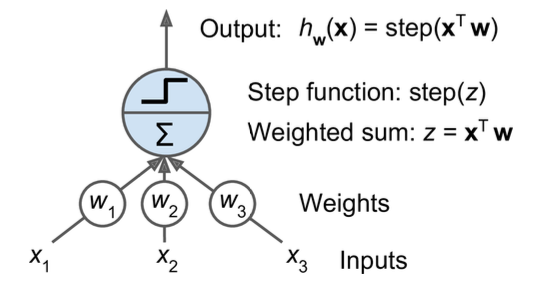
\includegraphics[width=0.45\textwidth]{Images/images_ch_4/perceptron.png}
    }
    \hfill
    \subfloat[Two-layer Perceptron: multiple TLUs stacked into an input and an output layer.\label{fig:two_layer_perceptron}]{
        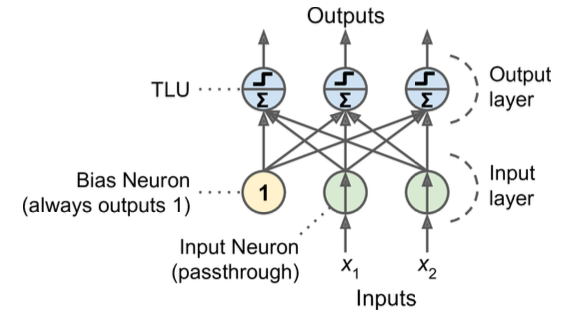
\includegraphics[width=0.45\textwidth]{Images/images_ch_4/two_layer_perceptron.png}
    }
    \caption{Perceptron architectures~\cite{geron2022hands}.}
    \label{fig:perceptrons}
\end{figure}

Moreover, an extra input called \textit{bias} is added ($x_0 = 1$): it is typically represented using a special type of neuron called a bias neuron, which just outputs 1 all the time. The bias shifts the activation boundary away from the origin.


\subsection{Forward propagation and backpropagation}
\label{subsec:forward_back}

The outputs of a layer of artificial neurons for several instances at once can be expressed through the following equation:

\begin{equation}
h_{\mathbf{W, b}}(\mathbf{X}) = \phi (\mathbf{X W} + \mathbf{b})
\end{equation}

\begin{itemize}
    \item As always, $\mathbf{X}$ represents the matrix of input features. It has one row per instance (e.g. spectrum), one column per feature (e.g. principal component).
    \item The weight matrix $\mathbf{W}$ contains all the connection weights except for the ones from the bias neuron. It has one row per input neuron, for the first layer it corresponds to the number of features, and one column per artificial neuron in the layer.
    \item The bias vector $\mathbf{b}$ contains all the connection weights between the bias neuron and the artificial neurons. It has one bias term per artificial neuron.
    \item The function $\phi$ is the activation function (e.g. step, sigmoid or ReLU).
\end{itemize}

Initially, perceptrons were trained by accounting for the error made by the network on a single training instance at a time. The weights of connections that helped reduce the error between prediction and ground truth were reinforced:

\begin{equation}
    w_{i,j}^{(\text{new})} = w_{i,j} + \eta \left( y_j - \hat{y}_j \right) x_i
    \label{eq:perceptron_update}
\end{equation}

where $x_i$ is the $i$-th input value of the current training instance, $\hat{y}_j$ is the predicted output of the $j$-th neuron, $y_j$ is the target output, and $\eta$ is the learning rate.
This learning method, solely based on the prediction for one instance, cannot be applied in networks with more than one hidden layer. This is due to not being able to isolate the role of a single connection in the prediction. The method, however, strongly resembles gradient descent.

In the case of networks with more than one hidden layer, called \textit{deep neural networks} (DNN), weights are updated through the \textit{backpropagation} algorithm, which is based on gradient descent. In two passes through the network (one forward, one backward), the backpropagation algorithm computes the gradient of the network's error with respect to every single model parameter:

\begin{enumerate}
    \item It takes one mini-batch at a time (for example containing 32 instances each), and it goes through the full training set multiple times. Each pass is called an \textit{epoch}.
    \item The output for every instance in the mini-batch is computed layer by layer. This is the \textit{forward pass}: it is like making predictions, but all intermediate results are preserved since they are needed for the backward pass.
    \item The algorithm measures the network's output error through a chosen loss function.
    \item It computes how much each connection in a layer contributed to the error. This is done analytically by applying the chain rule, from the output layer to the first one. This is the \textit{backward pass}.
    \item Finally, the algorithm performs a Gradient Descent step to tweak all the connection weights in the network, using the error gradients it just computed.
\end{enumerate}

More formally, for a network with $D$ layers, the loss is a composition:

\begin{equation}
    \mathcal{L} = L\!\Big(f^{(D)}\big(\cdots f^{(1)}(\mathbf{X};\, \mathbf{W}^{(1)}) \cdots;\, \mathbf{W}^{(D)}\big)\Big)
\end{equation}

where $L(\cdot)$ is the loss function and $f^{(i)}$ the full layer transformation for layer $i$ (i.e. $\phi\!\left(\mathbf{X}\mathbf{W}^{(i)} + \mathbf{b}^{(i)}\right)$).

The goal of backpropagation is to compute $\frac{\partial \mathcal{L}}{\partial \mathbf{W}^{(r)}}$ for every layer $r$, so that each weight matrix can be updated by gradient descent.

For layer $r$, preactivation $\mathbf{z}^{(r)}$ and activation $\mathbf{h}^{(r)}$ are:

\begin{equation}
    \mathbf{z}^{(r)} = \mathbf{h}^{(r-1)} \mathbf{W}^{(r)} + \mathbf{b}^{(r)}, \qquad \mathbf{h}^{(r)} = \phi\!\left(\mathbf{z}^{(r)}\right), \qquad \mathbf{h}^{(0)} = \mathbf{X}
\end{equation}

Applying the chain rule through all layers from $D$ back to $r$:

\begin{equation}
    \frac{\partial \mathcal{L}}{\partial \mathbf{W}^{(r)}} =
    \frac{\partial \mathcal{L}}{\partial \mathbf{h}^{(D)}} \cdot
    \frac{\partial \mathbf{h}^{(D)}}{\partial \mathbf{z}^{(D)}} \cdot
    \frac{\partial \mathbf{z}^{(D)}}{\partial \mathbf{h}^{(D-1)}} \cdot
    \frac{\partial \mathbf{h}^{(D-1)}}{\partial \mathbf{z}^{(D-1)}} \cdots
    \frac{\partial \mathbf{z}^{(r+1)}}{\partial \mathbf{h}^{(r)}} \cdot
    \frac{\partial \mathbf{h}^{(r)}}{\partial \mathbf{z}^{(r)}} \cdot
    \frac{\partial \mathbf{z}^{(r)}}{\partial \mathbf{W}^{(r)}}
      \label{eq:chain_rule}
\end{equation}

where each intermediate factor is

\begin{equation}
    \frac{\partial \mathbf{h}^{(k)}}{\partial \mathbf{z}^{(k)}} = \phi'\!\left(\mathbf{z}^{(k)}\right), \qquad
    \frac{\partial \mathbf{z}^{(k)}}{\partial \mathbf{h}^{(k-1)}} = \mathbf{W}^{(k)}, \qquad
\end{equation}

Finally, the full gradient can be rewritten in short form as follows

\begin{equation}
    \frac{\partial \mathcal{L}}{\partial \mathbf{W}^{(r)}} = \mathbf{h}^{(r-1)\top} \boldsymbol{\delta}^{(r)}
\end{equation}

where $\boldsymbol{\delta}^{(r)}$ is the \textit{backpropagated error signal} at layer $r$, which compresses all the intermediate derivatives in one term and is computed recursively, while $\mathbf{h}^{(r-1)\top}$ comes from the last term in \eqref{eq:chain_rule}.

Once the gradient is available, each weight matrix is updated by a step in the negative gradient direction:

\begin{equation}
    \mathbf{W}^{(r)}_{\text{new}} \leftarrow \mathbf{W}^{(r)} - \eta \, \frac{\partial \mathcal{L}}{\partial \mathbf{W}^{(r)}}
    \label{eq:gd_update}
\end{equation}

where $\eta > 0$ is the \textit{learning rate}, a hyperparameter controlling the step size. The same update applies to the bias vectors $\mathbf{b}^{(r)}$.

It is important to initialize all the hidden layers' connection weights randomly, otherwise all neurons will be identical, hence evolve in the same way. The model would be equivalent to having a single neuron per layer.


\subsection{Activation functions: sigmoid, ReLU}
\label{subsec:activation_functions}

In order for the backpropagation algorithm to work, the activation function must be changed from the step function to one such that its derivative is well-defined and nonzero everywhere, so that the gradient can always be computed and the weights updated effectively.
Furthermore, the activation functions must be non-linear. If they were linear, the transformation obtained by chaining them would be linear too (for example: $f(x)=x+1,\quad g(x)=2x-1 \quad\Rightarrow\quad f(g(x))=(2x-1)+1$). Without some non-linearity between layers, then even a deep stack of layers is equivalent to a single layer.

Multiple choices are possible for the activation function. In the model developed for this thesis, two functions were used: sigmoid and ReLU.

The \textit{sigmoid function} (also known as \textit{the logistic function}) was historically the first replacement for the step function.

\begin{equation}
    \sigma(z) = \frac{1}{1 + e^{-z}}
\end{equation}

It closely represents the firing rates of biological neurons and, due to squashing any input to a value $\in(0,1)$, it can be interpreted as a probability. It is thus particularly suited for the output layer, which is also where it was implemented in our model.

\begin{figure}[ht]
    \centering
    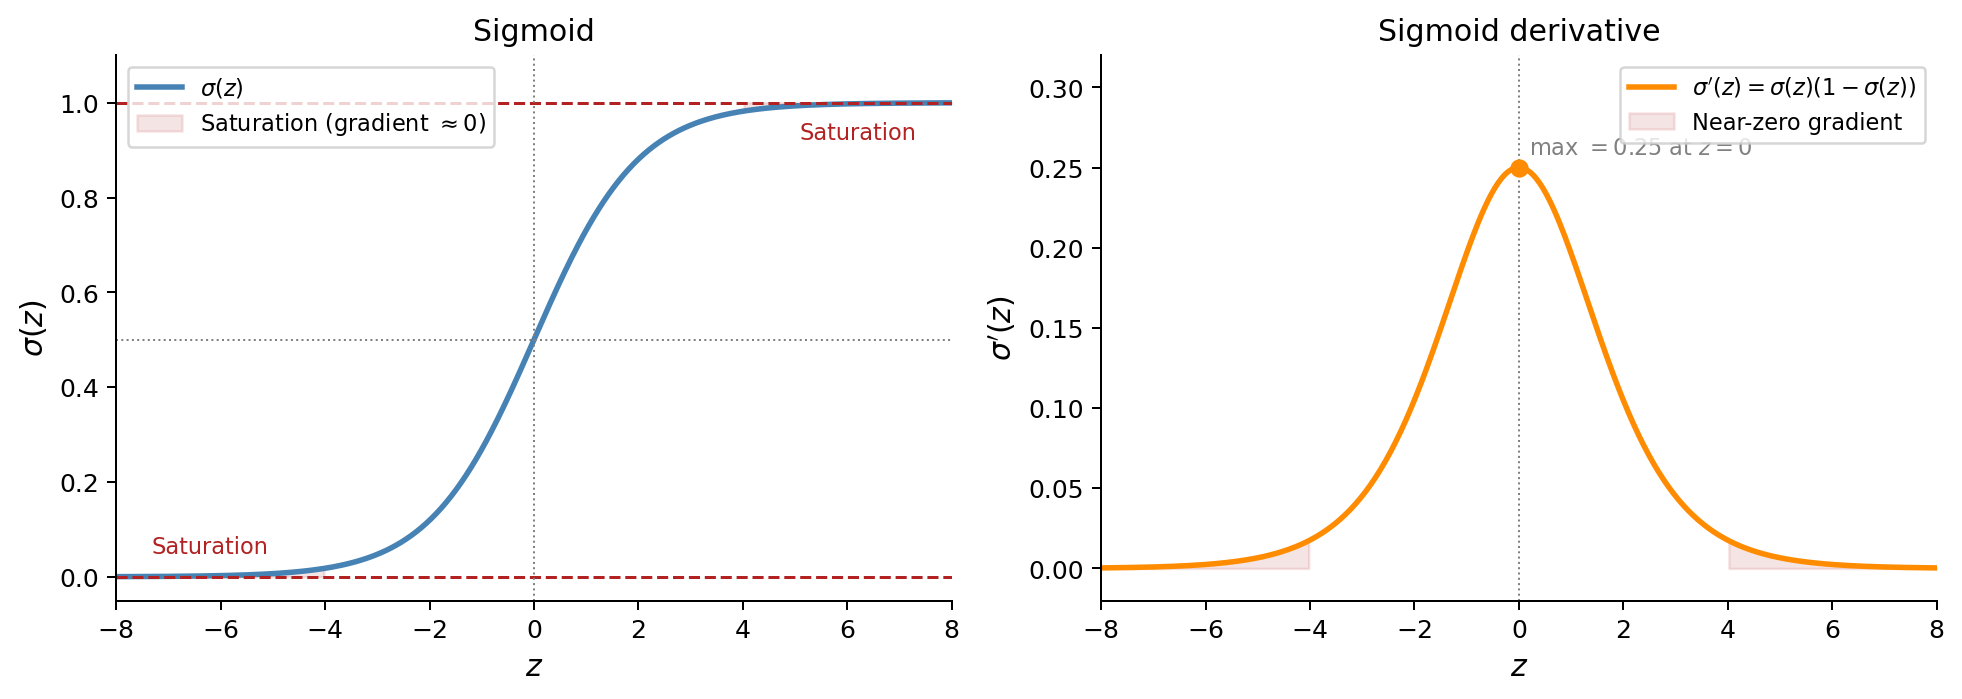
\includegraphics[width=0.8\textwidth]{Images/images_ch_4/sigmoid.png}
    \caption{Sigmoid function $\sigma(z)$ (left) and its derivative $\sigma'(z) = \sigma(z)(1-\sigma(z))$ (right). The shaded regions show the saturation zones where the gradient is nearly zero, slowing down learning through backpropagation.}
    \label{fig:sigmoid}
\end{figure}

The sigmoid shows nevertheless some problems.
Firstly, the saturation of the values of $\sigma(z)$ when $|z|\gg1$ causes the values of the gradient to shrink. Gradients can get progressively smaller as the algorithm progresses
down to the lower layers. As a result, the Gradient Descent update leaves the lower layer connection weights virtually unchanged, and training never converges to a good solution. This is called the \textit{vanishing gradients} problem.
To solve this problem, the hidden layers must have a non-saturating activation function.

The \textit{Rectified Linear Unit} (ReLU) is a simple alternative that doesn't saturate for positive values and has proven to be very effective in deep networks:

\begin{equation}
    \text{ReLU}(z) = \max(0, z)
\end{equation}

It is continuous but not differentiable at z = 0, which can make Gradient Descent bounce around, but it has the advantage of being very fast to compute, significantly reducing training time.
This has been the choice for the hidden layers for the ANN used for this thesis.

\begin{figure}[ht]
    \centering
    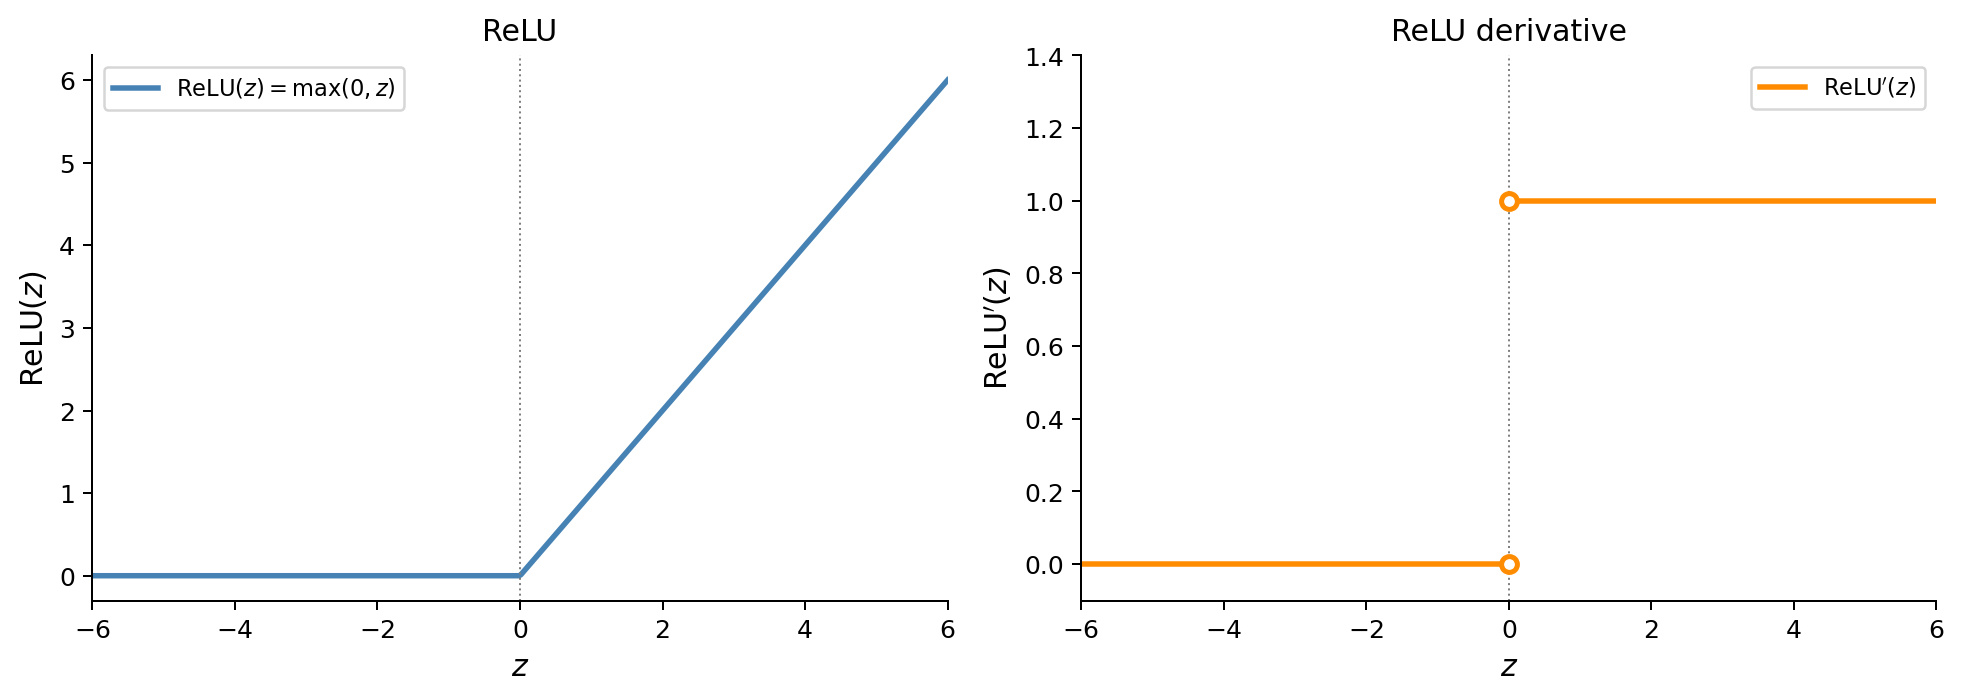
\includegraphics[width=0.8\textwidth]{Images/images_ch_4/relu.png}
    \caption{ReLU function (left) and its derivative (right). For $z < 0$ the output and gradient are both exactly zero --- the so-called \textit{dying ReLU} problem --- while for $z > 0$ the gradient is a constant 1, avoiding saturation.}
    \label{fig:relu}
\end{figure}

However, ReLU has the disadvantage that its derivative is zero for negative inputs. If all the training examples produce negative inputs to a given ReLU function, the parameters feeding into this ReLU during training cannot be improved, since the gradient with respect to the incoming weights is locally flat. This is known as the \textit{dying ReLU problem}.
To solve it, functions such as LeakyReLU (slightly tilted for $z<0$) exist, but they were not implemented in this work for simplicity.

% -----------------------------------------------------------------
% NEW §2.4.4 "Binary cross-entropy loss"
% <- OLD: Ch_4_ann.tex \subsection{Binary Cross-Entropy Loss} (same
%    title, capitalization style only; old 4.1.4 -> new 2.4.4).
% CLAUDIO: this subsection contains \cref{sec:binary_classification},
% which currently points at Ch_2_dataset.tex's "Binary labelling"
% section. Per the guide's migration map, that content splits into new
% §4.4 (operational definition) and §5.1 (the argument/results). You
% will need to decide which of the two this reference should now point
% to (guide item 4 flags exactly this: "due to the binary classification
% approach discussed in section 2.4 -> for the binary problems defined
% in §4.4"). Left as \cref{sec:binary_classification} verbatim, unresolved.
% -----------------------------------------------------------------
\subsection{Binary cross-entropy loss}
\label{subsec:bce}

As seen in the previous sections, Gradient Descent finds the best mapping from input to output by minimizing a \textit{Loss Function}.
Given a dataset $\{(\mathbf{x}_i, y_i)\}$ of input/output pairs, the \textit{loss function}~\cite{prince2023understanding} $L(\boldsymbol{\theta})$ returns a single number that describes the mismatch between the model predictions $f(\mathbf{x}_i, \boldsymbol{\theta})$ and their corresponding ground-truth outputs $y_i$, where $\boldsymbol{\theta}$ denotes the full set of learnable parameters (weights and biases).

Due to the \textit{binary classification} approach discussed in \cref{sec:binary_classification}, the ground-truths for this Artificial neural network will be integers $y_i\in\{0,1\}$. For more complex cases, \textit{multiclass classification}, with $K$ classes and $y_i\in\{0,1,\dots, K-1\}$, can be more useful.

To construct the loss function, a probability distribution based on the output space $y \in \{0,1\}$ must be chosen. A suitable choice is the Bernoulli distribution, which is defined on the domain $\{0,1\}$. This has a single parameter $\lambda \in [0,1]$ that represents the probability that $y$ takes the value one:

\begin{equation}
    \Pr(y|\lambda) = (1-\lambda)^{1-y} \cdot \lambda^y.
\end{equation}

The model $f[\mathbf{x}, \boldsymbol{\theta}]$ is set to predict the single distribution parameter $\lambda$. Since $\lambda$ can only take values in the range $[0,1]$, and the direct output of the last layer of the ANN is not bounded within said range, its output is passed through a function that maps $\mathbb{R} \rightarrow [0,1]$. This is why the output neuron has the \textit{sigmoid} as the activation function (\cref{subsec:activation_functions}).

Hence, the distribution parameter is predicted as $\lambda = \sigma(f[\mathbf{x}, \boldsymbol{\theta}])$. The likelihood is now:

\begin{equation}
    \Pr(y|\mathbf{x}) = (1 - \sigma[f[\mathbf{x}, \boldsymbol{\theta}]])^{1-y} \cdot \sigma[f[\mathbf{x}, \boldsymbol{\theta}]]^y.
\end{equation}

On the full training set $\{(\mathbf{x}_i, y_i)\}_{i=1}^{I}$, assuming independence across instances, it becomes:

\begin{equation}
    \prod_{i=1}^{I} \Pr(y_i | \mathbf{x}_i,
    \boldsymbol{\theta}) = \prod_{i=1}^{I} \left(1 - \sigma(f[\mathbf{x}_i,
    \boldsymbol{\theta}])\right)^{1-y_i} \cdot \sigma(f[\mathbf{x}_i,
    \boldsymbol{\theta}])^{y_i}
\end{equation}

since each factor $\Pr(y_i|\mathbf{x}_i, \boldsymbol{\theta}) \in (0,1)$, the product over $\sim10^6$ instances (Raman dataset's size) could underflow to zero. Taking the logarithm resolves this, transforming the product into a sum, which cannot underflow.

Likelihood is then maximized by minimizing its negative logarithm, since $\log$ is strictly monotonically increasing and thus preserves the location of the optimum.

\begin{equation}
    L[\boldsymbol{\theta}] =
    -\sum_{i=1}^{I} \left[(1-y_i)\log\left(1 - \sigma(f[\mathbf{x}_i,
    \boldsymbol{\theta}])\right) + y_i \log\left(\sigma(f[\mathbf{x}_i,
    \boldsymbol{\theta}])\right)\right]
\end{equation}

This is known as the \textit{binary cross-entropy loss}. The transformed model output $\sigma[f[\mathbf{x}, \boldsymbol{\theta}]]$ predicts the parameter $\lambda$ of the Bernoulli distribution. This represents the probability that $y = 1$, and it follows that $1 - \lambda$ represents the probability that $y = 0$.

When performing inference, the point estimate of $y$ is usually set such that $y = 1$ if $\lambda > 0.5$ and $y = 0$ otherwise.
However, in some cases it might be preferable to slightly tweak this to improve accuracy or recall, while considering that improving one will worsen the other (\cref{sec:evaluation_metrics}).


\subsection{Optimizers: from gradient descent to Adam}
\label{subsec:adam}

Training of the ANN can be substantially sped up by using a faster optimizer than the regular Gradient Descent.

Recalling that Gradient Descent, as in \cref{eq:gd_update}, simply updates the parameters $\boldsymbol{\theta}$ (weights and biases for all layers) by subtracting the gradient of the loss $\mathcal{L}$ multiplied by the learning rate $\eta$:
\begin{equation*}
    \boldsymbol{\theta} \leftarrow \boldsymbol{\theta} - \eta \, \frac{\partial \mathcal{L}}{\partial \boldsymbol{\theta}}
\end{equation*}
If the local gradient is tiny, convergence is very slow.

Unfortunately, loss functions for most nonlinear models are non-convex, meaning they have multiple local minima and saddle points. The algorithm can thus terminate in one
of the stationary points and there is no way of knowing whether there is a better solution elsewhere.

The final destination of a gradient descent algorithm is entirely determined by the starting point. \textit{Stochastic gradient descent} (SGD) attempts to solve this problem by adding some noise to the gradient at each step. There are multiple ways of introducing randomness in the algorithm.

Firstly, by dividing the training set in \textit{batches} and updating $\boldsymbol{\theta}$ after computing the gradient on every batch, the gradient will be representative of just a subset of the training set, and will tend to generalize better. SGD does not necessarily converge but, when close to the global minimum, all the data points will generally be well described by the model, so the gradients on all batches will be small. In practice, SGD is often applied with a \textit{learning rate schedule}. The learning rate $\eta$ starts at a high value and is decreased by a constant factor every $N$ epochs.

A possible improvement to SGD is to add a \textit{momentum} term. Parameters are updated with a weighted combination of the gradient computed from the current batch and the direction moved in the previous step:

\begin{align}
    \mathbf{m}_{t+1} &\leftarrow \beta \cdot \mathbf{m}_t + (1-\beta) \cdot \sum_{i \in \mathcal{B}_t} \frac{\partial \mathcal{L}_i(\boldsymbol{\theta}_t)}{\partial \boldsymbol{\theta}} \notag \\
    \boldsymbol{\theta}_{t+1} &\leftarrow \boldsymbol{\theta}_t - \eta \mathbf{m}_{t+1},
    \label{eq:momentum}
\end{align}

where $\mathbf{m}_t$ is the momentum at iteration $t$, $\beta \in [0,1)$ a hyperparameter that models friction ($\beta = 0 \Rightarrow$ high friction, $\beta \rightarrow 1 \Rightarrow$ no friction), $\eta$ the learning rate, and the gradient is calculated on the current mini-batch $\mathcal{B}_t$ \cite{geron2022hands, prince2023understanding}.

The gradient step is an exponentially-weighted sum of all the previous gradients, where the weights get smaller moving back in time. The overall effect is a smoother trajectory and reduced oscillatory behavior in valleys.

To further speed up the convergence in cases where the surface is much steeper in one direction than another (e.g. elongated bowl problem), it's possible to perform a pointwise \textit{normalization} of the gradient, in order to descend more directly towards the minimum (\cref{fig:gd_small_lr_grid,fig:gd_large_lr_grid,fig:norm_grad_grid}). However, since gradients are normalized, this method progresses with a fixed step, $\eta$, bouncing back and forth when near the minimum.

The combination of normalization and momentum gives the \textit{Adam Optimizer} \cite{geron2022hands, prince2023understanding}. The momentum term $\mathbf{m}_t$ from \cref{eq:momentum} is kept, and a second statistic $\mathbf{v}_t$ evolves in the same way, using another friction hyperparameter $\gamma \in [0,1)$. Rather than normalizing by the instantaneous gradient as above, Adam divides by a running estimate of its magnitude.

\begin{align}
    \mathbf{m}_{t+1} &\leftarrow \beta \cdot \mathbf{m}_t + (1-\beta) \cdot \sum_{i \in \mathcal{B}_t} \frac{\partial \mathcal{L}_i(\boldsymbol{\theta}_t)}{\partial \boldsymbol{\theta}} \notag \\
    \mathbf{v}_{t+1} &\leftarrow \gamma \cdot \mathbf{v}_t + (1-\gamma) \cdot \left(\sum_{i \in \mathcal{B}_t} \frac{\partial \mathcal{L}_i(\boldsymbol{\theta}_t)}{\partial \boldsymbol{\theta}}\right)^2,
    \label{eq:adam_moments}
\end{align}

where the square is taken elementwise.
Finally, $\boldsymbol{\theta}$ is updated using the momentum $\mathbf{m}_{t+1}$, normalized pointwise by the square root of the mean squared gradient $\mathbf{v}_{t+1}$:

\begin{equation}
    \boldsymbol{\theta}_{t+1} \leftarrow \boldsymbol{\theta}_t - \eta \cdot \frac{\mathbf{m}_{t+1}}{\sqrt{\mathbf{v}_{t+1}} + \epsilon},
    \label{eq:adam_update}
\end{equation}

where $\epsilon$ is a small constant added to avoid divergence when $\mathbf{v}_{t+1} \rightarrow 0$.
The result of \textit{Adam} is shown in \cref{fig:adam_grid}.

\begin{figure}[ht]
    \centering
    \subfloat[GD, $\eta=0.05$.\label{fig:gd_small_lr_grid}]{
        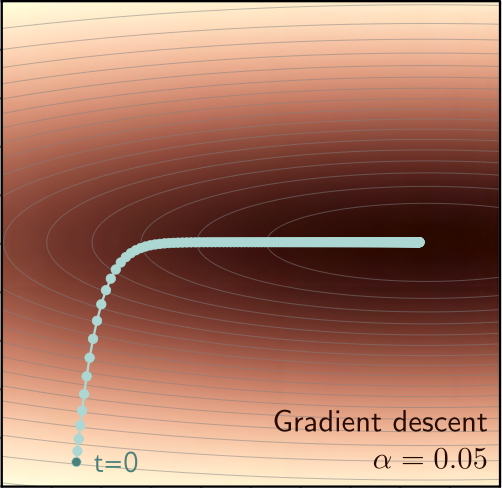
\includegraphics[width=0.4\textwidth]{Images/images_ch_4/grad_desc_1.png}
    }
    \hfill
    \subfloat[GD, $\eta=1.0$.\label{fig:gd_large_lr_grid}]{
        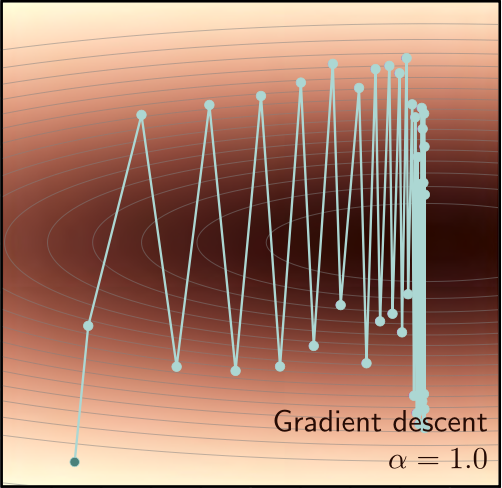
\includegraphics[width=0.4\textwidth]{Images/images_ch_4/grad_desc_2.png}
    }\\[1ex]
    \subfloat[Normalized gradients.\label{fig:norm_grad_grid}]{
        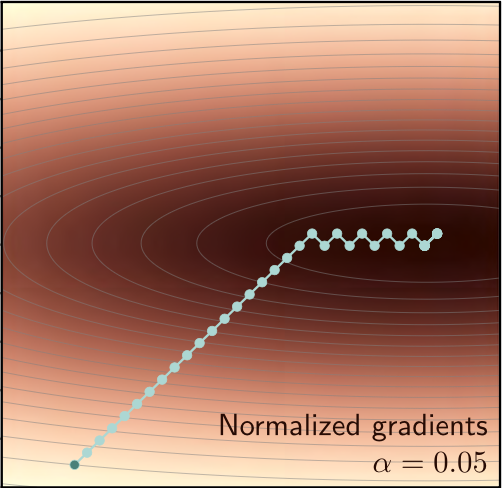
\includegraphics[width=0.4\textwidth]{Images/images_ch_4/norm_grad.png}
    }
    \hfill
    \subfloat[Adam.\label{fig:adam_grid}]{
        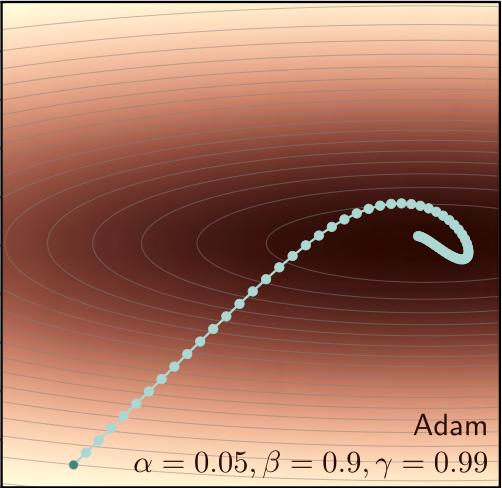
\includegraphics[width=0.4\textwidth]{Images/images_ch_4/adam.png}
    }
    \caption{Optimizer trajectories on an elongated bowl-shaped loss surface~\cite{prince2023understanding}.}
    \label{fig:optimizers_grid}
\end{figure}
